% !TeX encoding = UTF-8
\section{Results} \label{results}

For analysis 100 paintings from the \textit{Catalogue Raisonn{\'e}}
\cite{joosten1998} that matched the criteria were selected and scanned. The
scanned images were cropped so that no frame was visible. The images were then
processed by the detection program and subsequently checked for accuracy by
comparing the result with the original. The resulting dataset consists of 845
rectangles and their respective paintings.

Some explorative analysis about the use of color (\ref{color}) and ratios
(\ref{ratios}) was performed.

\subsection{Colors} \label{color}

On average Mondrian paintings consist of 78.3\% colors (red, blue, yellow) and
21.7\% non-colors (black, white) ($\sigma = 17.2\%$), see Figure
\ref{fig:colors-noncolors}. The distribution of different colors appears to be
fairly uniformly distributed as you can see in Figure \ref{colors-rby}.

\begin{figure}
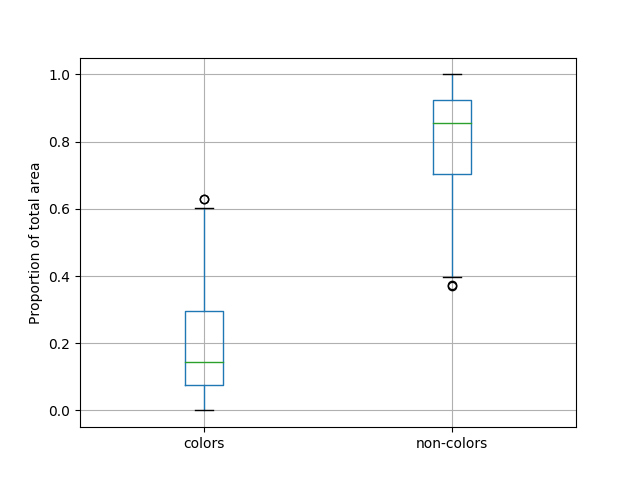
\includegraphics[width=\linewidth]{images/colors-non-colors.png}
\caption{Percentage of color/non-color of the total area}
\label{fig:colors-noncolors}
\end{figure}

\begin{figure}
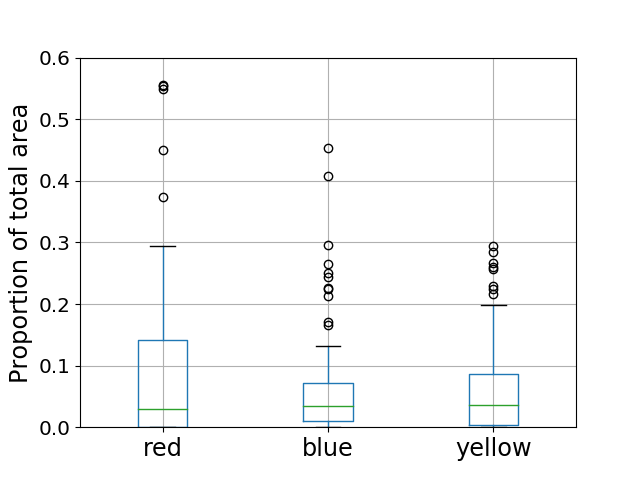
\includegraphics[width=\linewidth]{images/colors-rby.png}
\caption{Percentage of red, blue and yellow of the total area}
\label{fig:colors-rby}
\end{figure}

To see if different colors of rectangles have overall preferred positions in the
compositions, we assembled a dataset of all rectangles and their respective
positions, width and colors. We calculated the center of all of these rectangles
and plotted them by color. We also visualized the estimated probability density
function of the positions using Kernel density estimation. The first thing you
notice is that the color red appears to have a substantial bias to the top-left
corner. Similarly blue has a slighter bias to the bottom-right corner.

\begin{figure}
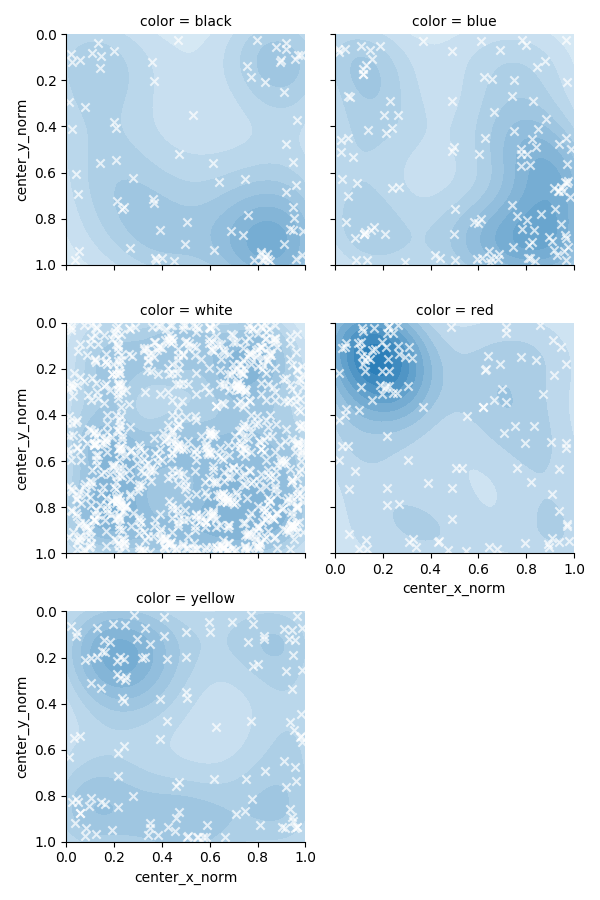
\includegraphics[width=\linewidth]{images/kernel-densities.png}
\caption{Scatter plots and KDE for each color}
\label{fig:kde}
\end{figure}

\subsection{Ratios} \label{ratios}

For all rectangles we calculated the aspect ratio of the longer to the shorter
side. Figure \ref{aspect-rects} shows the estimated probability density of the
ratios and Figure \ref{longer-x-shorter} shows all rectangles plotted by their
sides as well as lines for certain proposed ratios. The data does not show peaks
for the golden or silver ratio; instead it seems biased towards rectangles.

\begin{figure}
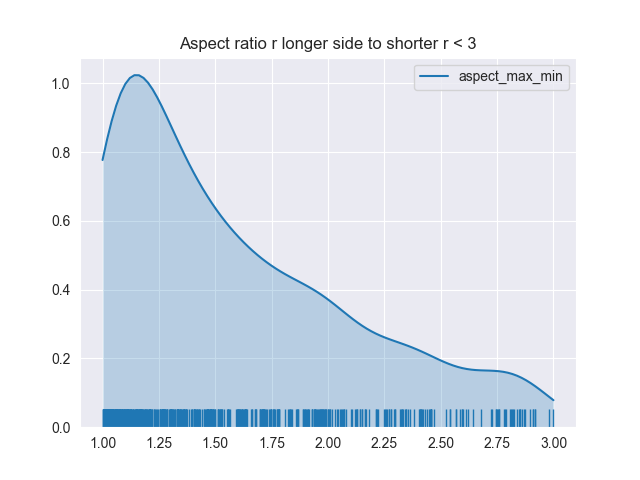
\includegraphics[width=\linewidth]{images/aspect-max-min-rects.png}
\caption{Rectangles ratio KDE}
\label{fig:aspect-rects}
\end{figure}

\begin{figure}
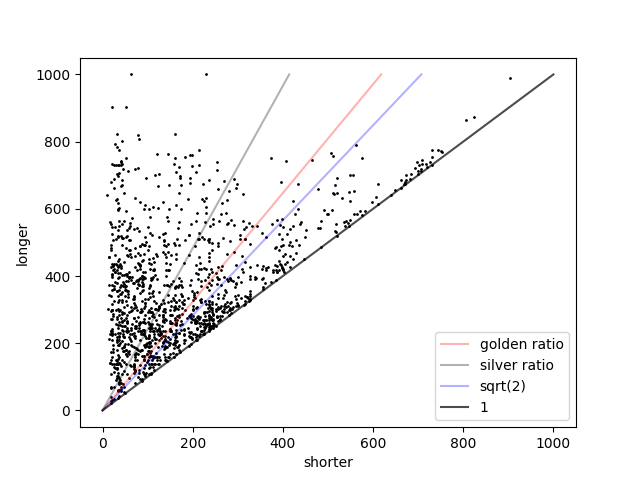
\includegraphics[width=\linewidth]{images/longer-x-shorter.png}
\caption{Rectangles longer side to shorter side}
\label{fig:longer-x-shorter}
\end{figure}


% TODO: Number of rectangles over time?
% TODO: How many paintings use all colors? How many with only one?
